% !TEX TS-program = pdflatex
% !TEX encoding = UTF-8 Unicode

% This is a simple template for a LaTeX document using the "article" class.
% See "book", "report", "letter" for other types of document.

\documentclass[11pt]{scrreprt} % use larger type; default would be 10pt
\linespread {1.25}\selectfont %1.25 da er von Haus aus 1.2 ist und 1,25 * 1,2 = 1,5 isch
\usepackage[utf8]{inputenc} % set input encoding (not needed with XeLaTeX)
%
%\setkomafont{chapter}{\Large\linespread{ 1}\sffamily\bfseries}
%\setkomafont{section}{\Large\linespread{ 1}\sffamily\bfseries}
%%% Examples of Article customizations
% These packages are optional, depending whether you want the features they provide.
% See the LaTeX Companion or other references for full information.

%%% PAGE DIMENSIONS
\usepackage{geometry} % to change the page dimensions
\geometry{a4paper} % or letterpaper (US) or a5paper or....
% \geometry{margin=2in} % for example, change the margins to 2 inches all round
% \geometry{landscape} % set up the page for landscape
%   read geometry.pdf for detailed page layout information

\usepackage{graphicx} % support the \includegraphics command and options

% \usepackage[parfill]{parskip} % Activate to begin paragraphs with an empty line rather than an indent

%%% PACKAGES
\usepackage[german]{babel}
\usepackage{helvet}
\usepackage{amsmath}
\usepackage{amssymb}
\usepackage{picinpar}
\usepackage{float}
\usepackage{epsfig}
\usepackage{graphicx}
\usepackage[german]{varioref}
\usepackage{longtable} %for tables langer than a page
\usepackage{booktabs} % for much better looking tables
\usepackage{array} % for better arrays (eg matrices) in maths
\usepackage{paralist} % very flexible & customisable lists (eg. enumerate/itemize, etc.)
\usepackage{verbatim} % adds environment for commenting out blocks of text & for better verbatim
\usepackage{subfig} % make it possible to include more than one captioned figure/table in a single float
% These packages are all incorporated in the memoir class to one degree or another...

%%% HEADERS & FOOTERS
\usepackage{fancyhdr} % This should be set AFTER setting up the page geometry //fancyhdr
\pagestyle{fancy} % options: empty , plain , fancy
%\fancyhf{}
\renewcommand{\headrulewidth}{0.5pt} % customise the layout...
%\lhead{}\chead{}\rhead{}
%\lfoot{}\cfoot{\thepage}\rfoot{}
%\lohead{\headmark}


%%%% SECTION TITLE APPEARANCE
%\usepackage{sectsty}
%\allsectionsfont{\sffamily\mdseries\upshape} % (See the fntguide.pdf for font help)
% (This matches ConTeXt defaults)


\setkomafont{chapter}{\rm\bf \large} %Größe der Kapitelüberschriften
\setkomafont{section}{\rm\bf\large} %Größe der UNterkapitelüberschriften 
\setkomafont{subsection}{\rm\bf\large} %Größe der UNterkapitelüberschriften 

%%% ToC (table of contents) APPEARANCE
\usepackage[nottoc,notlof,notlot]{tocbibind} % Put the bibliography in the ToC
\usepackage[titles,subfigure]{tocloft} % Alter the style of the Table of Contents
\renewcommand{\cftsecfont}{\rmfamily\mdseries\upshape}
\renewcommand{\cftsecpagefont}{\rmfamily\mdseries\upshape} % No bold!


%\usepackage[automark]{scrpage2}
%\pagestyle{scrheadings}


%%% END Article customizations



%%% The "real" document content comes below...

\title{Auswertung der Messungen über Kapazitätsänderung von Piezoelementen in Abhängigkeit von  eindimensionaler mechanischer Druckbelastung}
\author{Stephan Jobstmann}
\date {15. Mai 2012}
%\date{} % Activate to display a given date or no date (if empty),
         % otherwise the current date is printed 




\begin{document}
\maketitle
\tableofcontents
\def\chapterpagestyle{fancy}
\chapter{Einleitung}

\section{Motivation}

Ausschlaggebend für diese Messungen ist die Bestimmung von mechanischen Lastwechseln im niederfrequenten Bereich unter 4Hz. Genauer handelt es sich dabei um die Erfassung der Druckbelastung einer medizinischen Schienung eines verletzten Beines, mithilfe von piezoeletrischen Elementen. Bei diesen Bauelementen kann man anhand von drei Parametern Rückschlüsse auf die mechanische Belastung ziehen:
\begin{itemize}
\item Spannung,
\item Ladung,
\item Kapazität.
\end{itemize}
Dieses Protokoll bezieht sich auf die Untersuchung von Abhängigkeiten zwischen mechanischer Druckbelastung und elektrischer Kapazitätsänderung am Piezoelement.
\section{Aufgabenstellung und Versuchsaufbau}

Ziel dieser Versuchsreihe ist die Bestimmung der Kapazitätsänderung von piezoelektrischen Elementen bei mechanischer Druckbelastung. Dabei wird das Piezoelement elektrisch isoliert in einem Schraubstock belastet. Über Zuleitungen wird mit einem sogenannten LCR-Meter eine Vierdraht-Impedanz-Messung durchgeführt, die einzelnen Parameter hierfür werden bei den Versuchsreihen angegeben. Mithilfe einer Kraftmessdose, welche eine Vollmessbrücke mit Dehnmessstreifen beinhaltet, wird der angelegte mechanische Druck am Piezoelement abgeleitet. Da zu Messbeginn nur geringe Zusatzinformationen zu diesem Hilfsmittel vorhanden waren, geschahen alle Auswertungen in einem geringen Bereich unterhalb der Maximalbelastbarkeit von 250N. Weiter ist die angelegte Versorgungsspannung an der Messdose stets 10V DC. bei allen Messungen wurde ein LCR-Meter ISO-TECH LCR-821 zur Impedanzmessung und ein Fluke-Hand-Multimeter 179 zur Spannungsmessung verwendet. Als Spannungsquelle stand ein Hameg HM8142 bereit.

\section{Ergebnis}

Im Allgemeinen lassen sich aufgrund der getätigten Messungen folgende Aussagen treffen:
\begin{itemize}
\item
Die Kapazitätsänderung der Piezoelemente unter Last stellt keine hinreichend reproduzierbare Methode zur Messung von mechanischer Druckbelastung dar. Aufgrund der massiv einwirkenden parasitären Effekte, seien es Veränderungen der Luftfeuchte, Temperaturschwankungen oder pyroelektrische Einflüsse, konnten keine eindeutig wiederholbaren Werte erzielt werden.
\item
Die Werkstoffstabilität ist auch in Frage zu stellen. Während der Messung ist ein Element unter Belastung zu Bruch gegangen.
\item
Weiter lassen sich die Ergebnisse der einzelnen Prüflinge unterscheiden:
\begin{itemize}
\item
CeramTec, P502, einschichtiger Piezo: Unter steigender Belastung verläuft die dazu korrespondierende Kapazitätskurve wie eine Exponentialfunktion mit negativem Exponenten. Weiter ist dieser während der Messung bei einer nicht mehr nachvollziehbaren Belastung zerbrochen. Die Reproduzierbarkeit einzelner Messergebnisse ist nahezu ausgeschlossen.
\item
CeramTec, P505, Mehrschichtiger Piezo: Auch bei diesem Piezoelement ver-läuft unter steigender Belastung die dazugehörige Kapazitätskurve monoton fallend. Weiter wurde auch hier eine hohe Abhängigkeit von äußeren Einflüssen festgestellt.
\item
Elliptec, Mehrschichtiger Piezo: Bei diesem Stack ergab sich eine mit dem Druck steigende Kapazitätskurve. Allerdings erschwerten auch hier parasitäre Effekte eine eventuelle Reproduzierbarkeit.
\end{itemize}
\end{itemize}


\chapter{Messungen}

\section{Sonox P502} 
Bei diesem Piezobaustein handelt es sich um ein einfaches, nicht mehrschichtiges Element. Die nachfolgenden Messungen untersuchten das Verhalten der Kapazität unter mechanischer Druckbelastung entlang der elektrischen Feldorientierung. Entgegen der Erwartung, dass die Kapazität mit steigender Druckbelastung ebenfalls steigt, verhält sich diese mehr wie eine Exponentialfunktion mit negativen Exponenten. Dies ist in nahezu allen folgenden Graphen der kommenden Unterkapitel nachzuvollziehen.
%%%%%%%%%%%%%Kapazität über steigender Druckbelastung%%%%%%%%%%%%%%%
\subsection{Kapazität über steigender Druckbelastung}
Diese Messung zeigt das kapazitive Verhalten des Piezoelements Sonox P502. Bei den Messwerten wird die Kapazität über die angelegte Kraft, bzw. die Spannung an der Kraftmessdose, aufgetragen, wie in Tabelle \vref{tab:2.1} und Abbildung \vref{fig:2.1} nachzuvollziehen ist. Speisefrequenz der Impedanzmessung war 500Hz bei 1V Amplitude.
\setlongtables
\begin{longtable}{| l | l | l |}
\caption{Messung 1}\\
\hline
$U_{diff}$ in mV&$C_{diff}$ in nF&$C_{Piezo}$ in nF\\
\hline
\endfirsthead
\hline
$U_{diff}$ in mV&$C_{diff}$ in $nF$&$C_{Piezo}$ in nF\\
\hline
\endhead
\hline
\multicolumn{3}{|c|}{Fortsetzung auf der nächsten Seite}\\
\hline
\endfoot
\hline \hline
\endlastfoot
\hline
\label{tab:2.1}%
0.02&-0.01795&\\
0.50&-0.0235&\\
0.94&-0.02212&\\
1.48&-0.0235&0.9766\\
1.93&-0.0244&0.9754\\
2.49&-0.02529&0.9748\\
3.00&-0.02801&0.9716\\
3.60&-0.0294&0.9705\\
4.10&-0.02995&0.96981\\
4.56&-0.03057&0.96935\\
5.00&-0.03137&0.96858\\
5.51&-0.03184&0.96811\\
6.11&-0.03231&0.96766\\
\end{longtable}
\begin {figure}[htbp]
      \begin{center}
        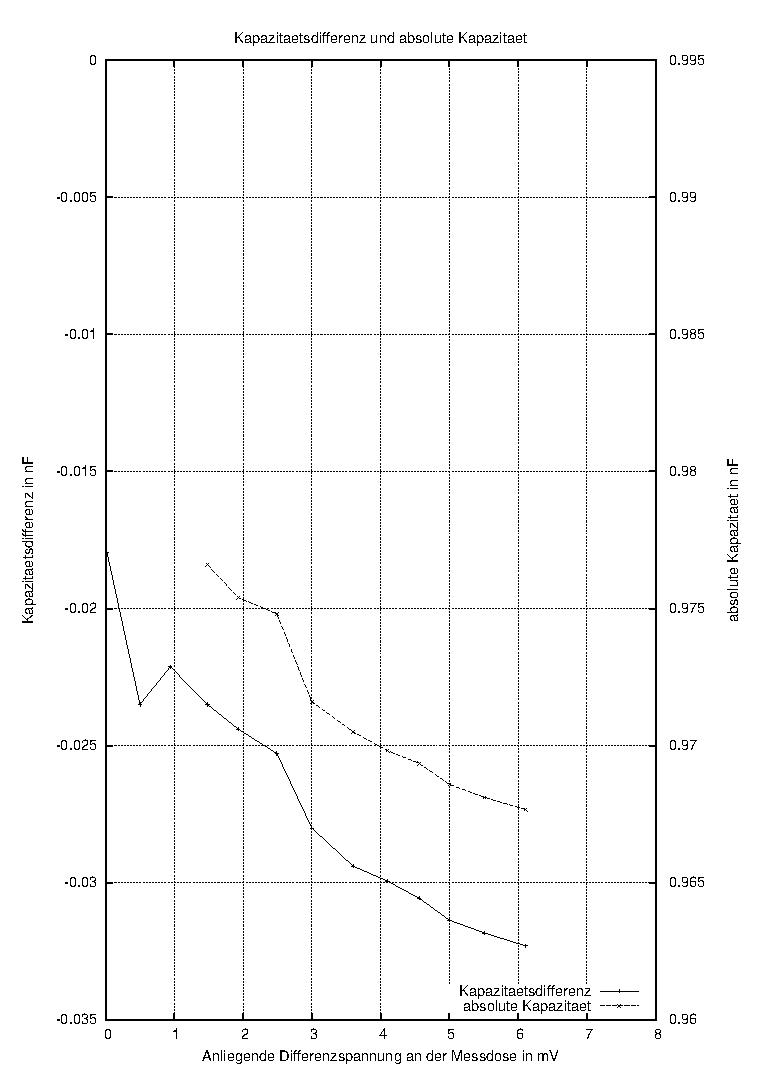
\includegraphics{tabelle2_1_1}
      \end{center}
\caption{Messung 1}
\label{fig:2.1}
\end{figure}

%%%%%%%%%%%Kapazität über statischer Druckbelastung%%%%%%%%%%%%%%%
\subsection{Kapazität über statischer Druckbelastung}
Durch die bei der ersten Messung stets ändernden Kapazitäten während einer Druckvorgabe wird dieser Versuch zur Untersuchung bei statischer Belastung angesetzt. Durch die Beobachtung der sinkenden Spannungsdifferenz (der Kraftmessdose) über die Zeit lässt sich die auftretende Kapazitätsänderung (des Piezoelements) auf die elastischen Kunststoffbacken des Schraubstocks zurückführen. Die Werte bzw. die grafische Auswertung ist hierbei aus der Tabelle \vref{tab:2.2} und dem Graphen aus Abbildung \vref{fig:2.2} zu entnehmen. \\
Aufgrund eines Gegenvergleichs lässt sich an dieser Stelle bereits sagen, dass die sich verringernden Werte auf die fortwährende Entspannung der Kunststoffbacken des Schraubstocks zurückführen lässt.

\setlongtables
\begin{longtable}{| l | l | l |}
\caption{Messung 2 }\\
\hline
Uhrzeit&$U_{diff}$ in mV&$C_{Piezo}$ in nF\\
\hline
\endfirsthead
\hline
Uhrzeit&$U_{diff}$ in mV&$C_{Piezo}$ in nF\\
\hline
\endhead
\hline
\multicolumn{3}{|c|}{Fortsetzung auf der nächsten Seite}\\
\hline
\endfoot
\hline \hline
\endlastfoot
\hline
\label{tab:2.2}%
09:50:00&10.12&0.9734\\
10:20:00&9.59&0.9662\\
11:40:00&9.37&0.96311\\
\end{longtable}

\begin {figure}[htbp]
      \begin{center}
        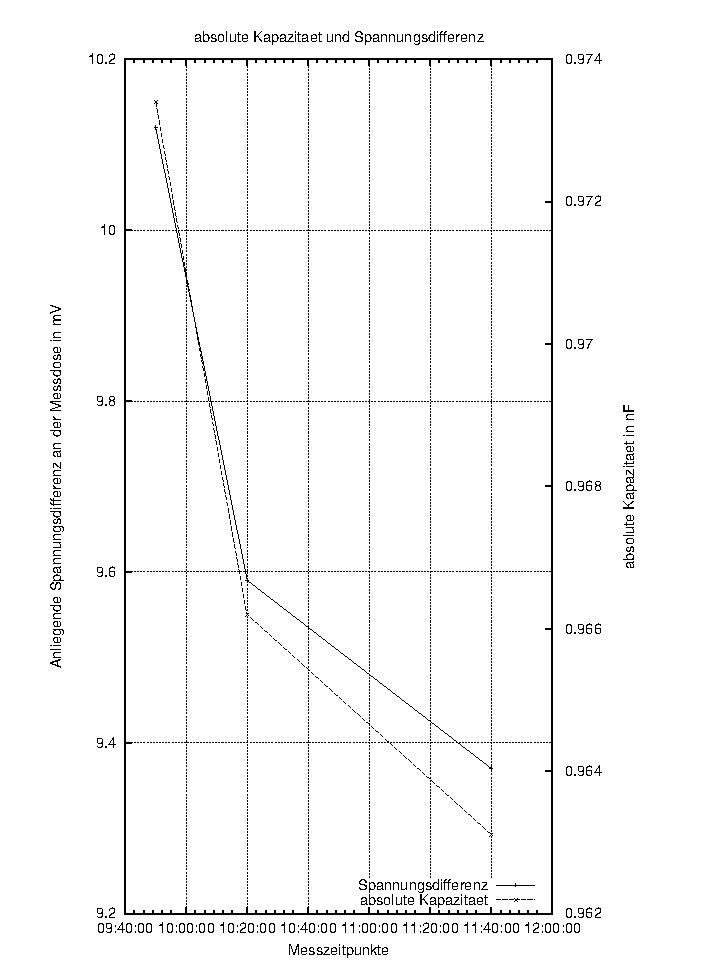
\includegraphics{tabelle2_1_2}
      \end{center}
\caption{Messung 2}
\label{fig:2.2}
\end{figure}
\newpage
%%%%%%%%%%%%%%Weitere Messung mithilfe des Maschinenschraubstocks%%%%%%%%%%%%%
\subsection{Weitere Messung mithilfe des Maschinenschraubstocks}
Bei vorhergehenden Messungen ergab sich der Verdacht, dass die Werte aufgrund der nicht konstanten Druckbelastung durch die Spannvorrichtung verfälscht worden sind. Darum ist diese Messreihe mit einem schweren Maschinenschraubstock mit Stahlbacken erstellt worden. Hierbei wurde zusätzlich noch der Einfluss eines Parallelwiderstands untersucht. Allerdings wurden die Messungen jeweils nach einer Abschätzung der auftretenden Messwertdifferenz abgebrochen, da dies nicht als zielführend erschien. Zum Sicherstellen dieser Annahme wurde jeweils noch ein Messwert bei einer Druckbelastung von einer äquivalenten Spannung von 10mV aufgenommen. Diese ergaben keine feststellbaren Unterschiede zu den letzten dokumentierten Werten. Bei den Messungen wurde jeweils eine Entspannungsphase der Belastungsvorrichtung von 2 Minuten bei jedem Messschritt eingehalten. Die erzielten Messergebnisse sind in den Tabellen \vref{tab:2.3} und \vref{tab:2.4} ersichtlich. Anhand der Abbildung \vref{fig:2.3} lässt sich die unveränderte Charakteristik des Verhaltens unter Last nachvollziehen. Die Skalierung wurde hier zur Veranschaulichung angepasst. 

\setlongtables
\begin{longtable}{| l | l |}
\caption{Messung 3; mit 100k$\Omega$ Parallelwiderstand}\\
\hline
$U_{diff}$ in mV&$C_{Piezo}$ in nF\\
\hline
\endfirsthead
\hline
$U_{diff}$ in mV&$C_{Piezo}$ in nF\\
\hline
\endhead
\hline
\multicolumn{2}{|c|}{Fortsetzung auf der nächsten Seite}\\
\hline
\endfoot
\hline \hline
\endlastfoot
\hline
\label{tab:2.3}%
0.44&0.9719\\
0.97&0.9685\\
1.75&0.9675\\
2.36&0.9665\\
3.00&0.9654\\
3.53&0.9645\\
4.03&0.9643\\
4.53&0.963\\
5.05&0.9625\\
5.78&0.9626\\
6.38&0.9625\\
\end{longtable}

\setlongtables
\begin{longtable}{| l | l |}
\caption{Messung 4; ohne Parallelwiderstand}\\
\hline
$U_{diff}$ in mV&$C_{Piezo}$ in nF\\
\hline
\endfirsthead
\hline
$U_{diff}$ in mV&$C_{Piezo}$ in nF\\
\hline
\endhead
\hline
\multicolumn{2}{|c|}{Fortsetzung auf der nächsten Seite}\\
\hline
\endfoot
\hline \hline
\endlastfoot
\hline
\label{tab:2.4}%
0.64&0.9683\\
1.26&0.9640\\
1.75&0.9620\\
2.40&0.9603\\
2.87&0.9587\\
3.88&0.9570\\
4.38&0.9540\\
5.22&0.9538\\
\end{longtable}

\begin {figure}[htbp]
      \begin{center}
        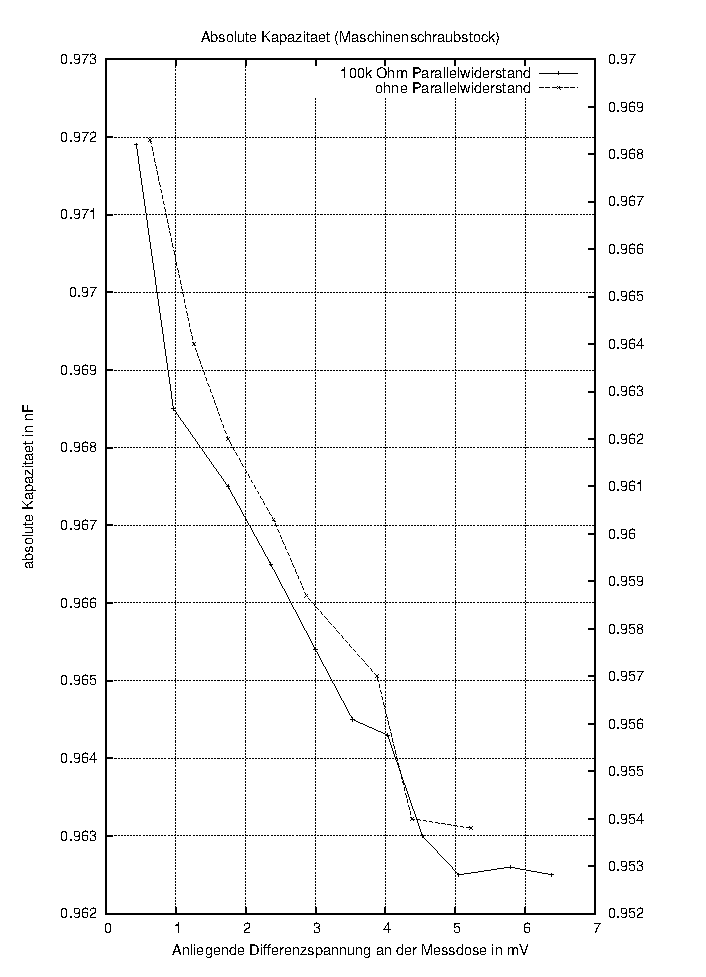
\includegraphics{tabelle2_1_3}
      \end{center}
\caption{Messung 3 und 4}
\label{fig:2.3}
\end{figure}

\newpage
\subsection{Messung mit anderer Impedanzmessfrequenz}
Da generell eine Veränderung des Impedanzverhaltens über die Frequenz bei Piezoelementen zu erwarten ist, wurde diese Messung mit halber Frequenz angestrebt. Allerdings sind die sich ergebenden Unterschiede so gering, dass sie von parasitären Effekten überlagert werden und die äußeren Umwelteinflüsse (Temperatur, relative Luftfeuchte) maßgebend für die Ergebnisse sind. Die erzielten Werte sind der Tabelle \vref{tab:2.5} zu entnehmen. Die weiterhin fallende Kapazitätskurve über die Druckbelastung ist in Abbildung \vref{fig:2.4} ersichtlich.\\
Um eine weitere qualitative Aussage über das Frequenzverhalten treffen zu können, wurde empirisch die erste Resonanzfrequenz des Piezoelements ermittelt. Hierzu wurde ein Frequenzgenerator mit manuellem Sweep betrieben und mithilfe eines Shuntwiderstands der Strom in Serie auf Extrema beobachtet. Nach dieser Messung lässt sich ein Resonanzverhalten bei ca. 2.84 MHz feststellen. Aufgrund des weiten Abstands zur Messfrequenz kann man weitere Schlüsse ziehen. Daraus lässt sich auch die unveränderte Charakteristik der vorhergehenden Messung bestätigen.

\setlongtables
\begin{longtable}{| l | l |}
\caption{Messung 5; 1kHz Messfrequenz}\\
\hline
$U_{diff}$ in mV&$C_{Piezo}$ in nF\\
\hline
\endfirsthead
\hline
$U_{diff}$ in mV&$C_{Piezo}$ in nF\\
\hline
\endhead
\hline
\multicolumn{2}{|c|}{Fortsetzung auf der nächsten Seite}\\
\hline
\endfoot
\hline \hline
\endlastfoot
\hline
\label{tab:2.5}%
0.4&0.9705\\
1.4&0.9709\\
2.0&0.9690\\
3.0&0.9681\\
3.8&0.9675\\
5.0&0.9670\\
\end{longtable}

\begin {figure}[htbp]
      \begin{center}
        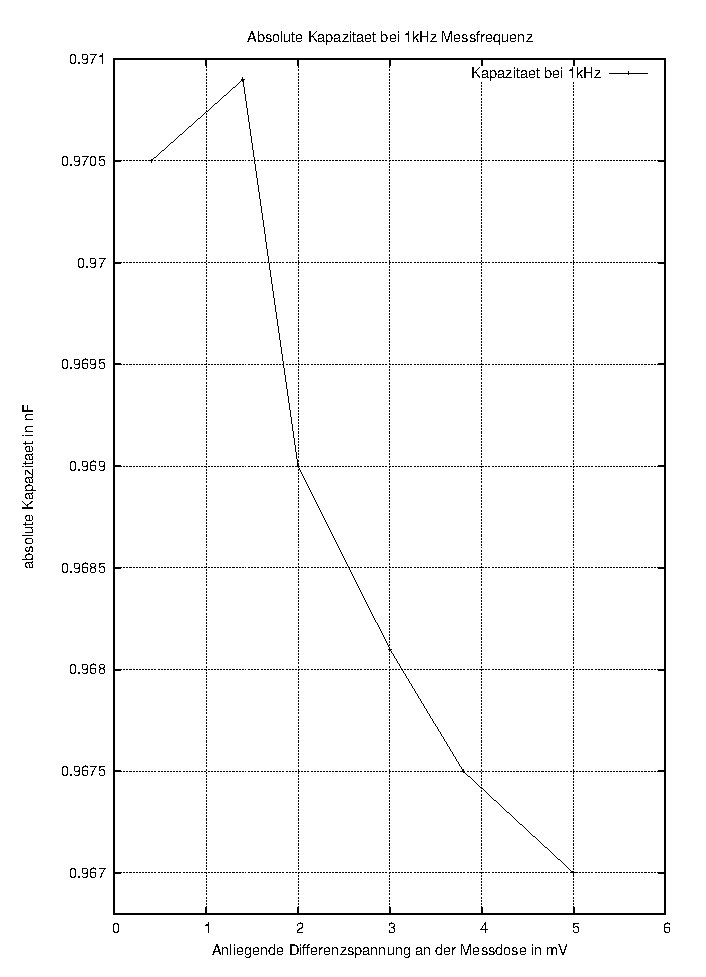
\includegraphics{tabelle2_1_4}
      \end{center}
\caption{Messung 5}
\label{fig:2.4}
\end{figure}

\newpage
\section{Bürklin Piezo-Stack von Elliptec}
Da die vorhergehenden Messungen mit dem einfach aufgebauten Piezoelement nicht die erforderlichen Resultate bezüglich Charakteristik und Reproduzierbarkeit brachten, wurde nun eine Versuchsreihe mit gestapelten Piezoelementen angestrebt. Der Messaufbau blieb weiterhin derselbe, d.h. mithilfe eines Schraubstocks mit Kunststoffbacken wurde eine mechanische Druckbelastung an den Piezostack (im Folgenden auch Stack genannt) und einer Kraftmessdose in Serie angelegt. Beim verwendeten LCR-Meter wurden folgende Parameter eingestellt:
\begin{itemize}
\item 1kHz
\item 1V
\item R.H. off
\item C.V. off
\item int B. off
\end{itemize}
Weiter wurden bei diesen Messungen die Zuleitungen nicht auf dem Stack direkt aufgelötet, da dies den Messvorgang an sich unmöglich gemacht hätte. Stattdessen wurden Keramikträger als lose Verbindung der Messleitungen zum Piezoelement vewendet. Dadurch kann es bei geringer mechanischer Belastung zu Verfälschungen gekommen sein, da der Kontakt zwischen Stack und Keramik unzureichend war.
\subsection{Messung Piezo-Stack, ohne Entladungsmaßnahme}
Bei dieser ersten Vermessung des kapazitiven Verhaltens des Piezostacks unter Druckbelastung in elektrischer Feldrichtung wurde eine Entspannungszeit der Kunststoffbacken des Schraubstocks von 2 Minuten berücksichtigt. Es wurde lediglich der Piezo ohne zusätzlichen Parallel- oder Serienwiderstand vermessen. Die auffällig abweichenden Anfangswerte in Abbildung \vref{fig:2.6} sind auf den schlechten Kontakt zwischen Keramikplättchen und Stack bei geringer Druckbelastung zurückzuführen. Die aufgenommenen Werte sind in Tabelle \vref{tab:2.6} zu finden.

\setlongtables
\begin{longtable}{| l |l| l |}
\caption{Messung 6; Piezostack; Einführende Messung}\\
\hline
$U_{diff}$ in mV&$C_{Piezo}$ in nF&$R_{Parallel}$ in k$\Omega$\\
\hline
\endfirsthead
\hline
$U_{diff}$ in mV&$C_{Piezo}$ in nF&$R_{Parallel}$ in k$\Omega$\\
\hline
\endhead
\hline
\multicolumn{3}{|c|}{Fortsetzung auf der nächsten Seite}\\
\hline
\endfoot
\hline \hline
\endlastfoot
\hline
\label{tab:2.6}%
0.7&253.25&2.39\\
1.2&270.00&8.01\\
1.9&271.39&15.48\\
2.9&271.83&16.98\\
3.6&271.98&17.40\\
4.5&272.22&17.42\\
6.1&272.47&15.80\\
7.0&272.70&17.72\\
8.0&272.83&18.28\\
9.4&273.16&18.30\\
10.9&273.62&17.21\\
\end{longtable}

\begin {figure}[htbp]
      \begin{center}
        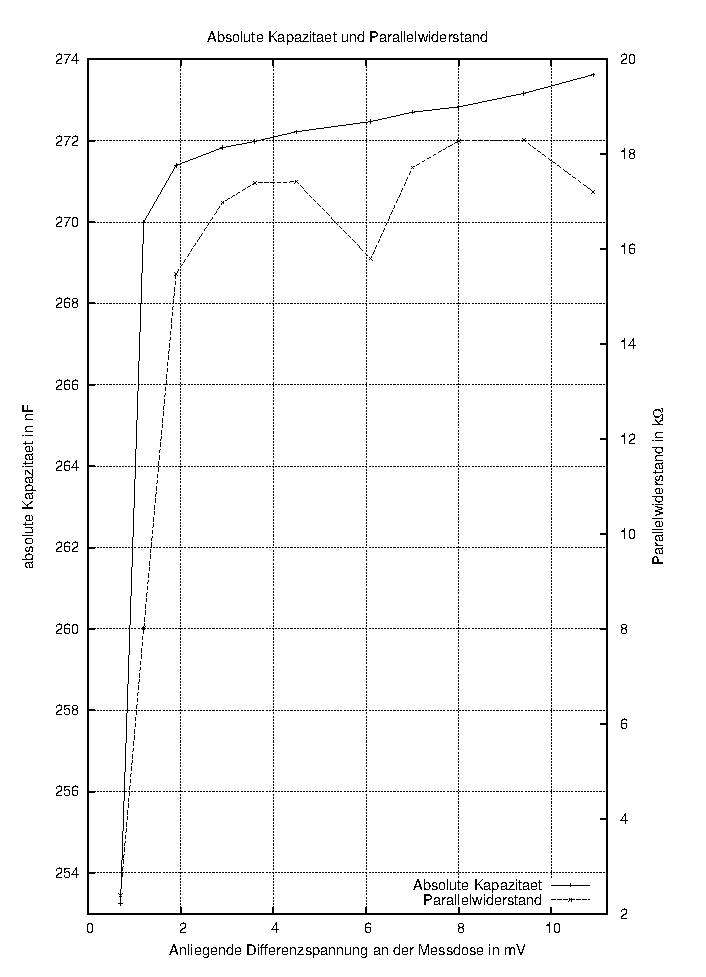
\includegraphics{tabelle2_2_1}
      \end{center}
\caption{Messung 6; Einführende Messung Piezostack}
\label{fig:2.6}
\end{figure}

\newpage
\subsection{Messung Piezo-Stack, mit Entladung, ohne Setz-Zeit}
Um störende, vom Stack selbst erzeugte Ladungsquellen ausschließen zu können, wurde diese Messung in jeweils zwei Schritten ausgeführt. Beim ersten Schritt wird die Kraft angelegt und der Piezo-Stack kurzgeschlossen, um so möglicherweise erzeugte Ladungen zu eliminieren. Als zweiten Schritt wird mithilfe des LCR-821 eine Impedanzmessung durchgeführt. Diese beiden Schritte wurden je unter 30 Sekunden durchgeführt, um ein möglichst isochrones Ergebnis zu erhalten. 
Weiter wurde die Messung ein zweites Mal durchgeführt, um eine Aussage über die Reproduzierbarkeit treffen zu können. Beim Vergleich der Graphen in Abbildung \vref{fig:2.7} wird deutlich, dass selbst bei unmittelbar aufeinanderfolgenden Messungen keine zureichende Wiederholbarkeit der Messvorgänge erreicht werden kann. Die korrespondierenden Werte beider Messungen sind in Tabelle \vref{tab:2.7} zu finden.
Um Rückschlüsse auf das $\varepsilon$ des Piezomaterials zu ermöglichen, wurde der Parallelwiderstand bei diesem Messvorgang mit aufgezeichnet. Die Resultate sind in der Tabelle \vref{tab:2.8} und Abbildung \vref{fig:2.8} ersichtlich.

\setlongtables
\begin{longtable}{| l | l | l | l |}
\caption{Messung 7; Piezostack; mit Entladung, ohne Setz-Zeit; Kapazität}\\
\hline
\multicolumn{2}{|c|}{Messung 1} &\multicolumn{2}{|c|}{Messung 2}\\
\hline
$U_{diff}$ in mV&$C_{Piezo}$ in nF&$U_{diff}$ in mV&$C_{Piezo}$ in nF\\
\hline
\endfirsthead
\hline
\multicolumn{2}{|c|}{Messung 1} &\multicolumn{2}{|c|}{Messung 2}\\
\hline
$U_{diff}$ in mV&$C_{Piezo}$ in nF&$U_{diff}$ in mV&$C_{Piezo}$ in nF\\
\hline
\endhead
\hline
\multicolumn{4}{|c|}{Fortsetzung auf der nächsten Seite}\\
\hline
\endfoot
\hline \hline
\endlastfoot
\hline
\label{tab:2.7}%
0.15&266.66&0.49&269.02\\
1.15&267.14&1.55&268.98\\
2.55&267.72&2.82&269.26\\
3.24&267.93&3.63&269.36\\
4.39&268.6&4.60&269.55\\
5.10&268.88&5.57&269.78\\
6.14&269.32&6.39&269.90\\
7.55&268.95&7.74&270.25\\
8.24&270.16&8.40&270.40\\
9.82&270.71&9.52&270.70\\
10.45&270.76&10.49&270.84\\
\end{longtable}

\begin {figure}[htbp]
      \begin{center}
        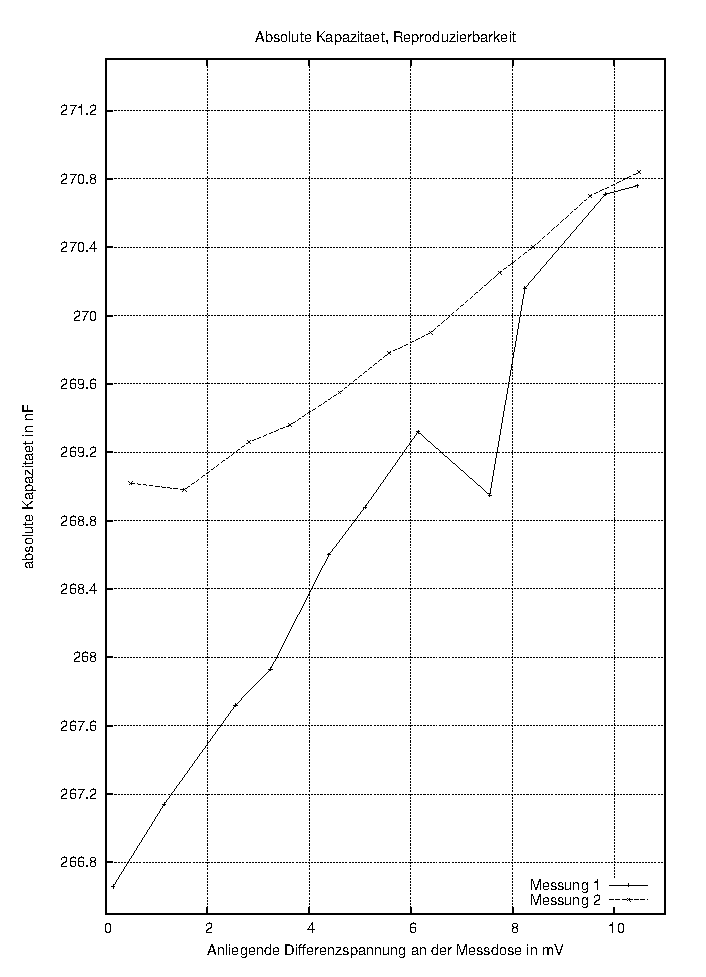
\includegraphics{tabelle2_2_2}
      \end{center}
\caption{Messung 7; mit Entladung, ohne Setz-Zeit; Piezostack; Kapazität}
\label{fig:2.7}
\end{figure}

\setlongtables
\begin{longtable}{| l | l | l | l |}
\caption{Messung 8; Piezostack; mit Entladung, ohne Setz-Zeit; Parallelwiderstand}\\
\hline
\multicolumn{2}{|c|}{Messung 1} &\multicolumn{2}{|c|}{Messung 2}\\
\hline
$U_{diff}$ in mV&$R_{Parallel}$ in k$\Omega$&$U_{diff}$ in mV&$R_{Parallel}$ in k$\Omega$\\
\hline
\endfirsthead
\hline
\multicolumn{2}{|c|}{Messung 1} &\multicolumn{2}{|c|}{Messung 2}\\
\hline
$U_{diff}$ in mV&$R_{Parallel}$ in k$\Omega$&$U_{diff}$ in mV&$R_{Parallel}$ in k$\Omega$\\
\hline
\endhead
\hline
\multicolumn{4}{|c|}{Fortsetzung auf der nächsten Seite}\\
\hline
\endfoot
\hline \hline
\endlastfoot
\hline
\label{tab:2.8}%
0.15&16.53&0.49&17.42\\
1.15&19.24&1.55&18.38\\
2.55&19.25&2.82&18.68\\
3.24&19.58&3.63&18.63\\
4.39&19.19&4.60&18.72\\
5.10&19.15&5.57&17.72\\
6.14&18.93&6.39&18.70\\
7.55&18.62&7.74&18.65\\
8.24&18.58&8.40&17.63\\
9.82&18.38&9.52&18.55\\
10.45&18.51&10.49&18.60\\
\end{longtable}

\begin {figure}[htbp]
      \begin{center}
        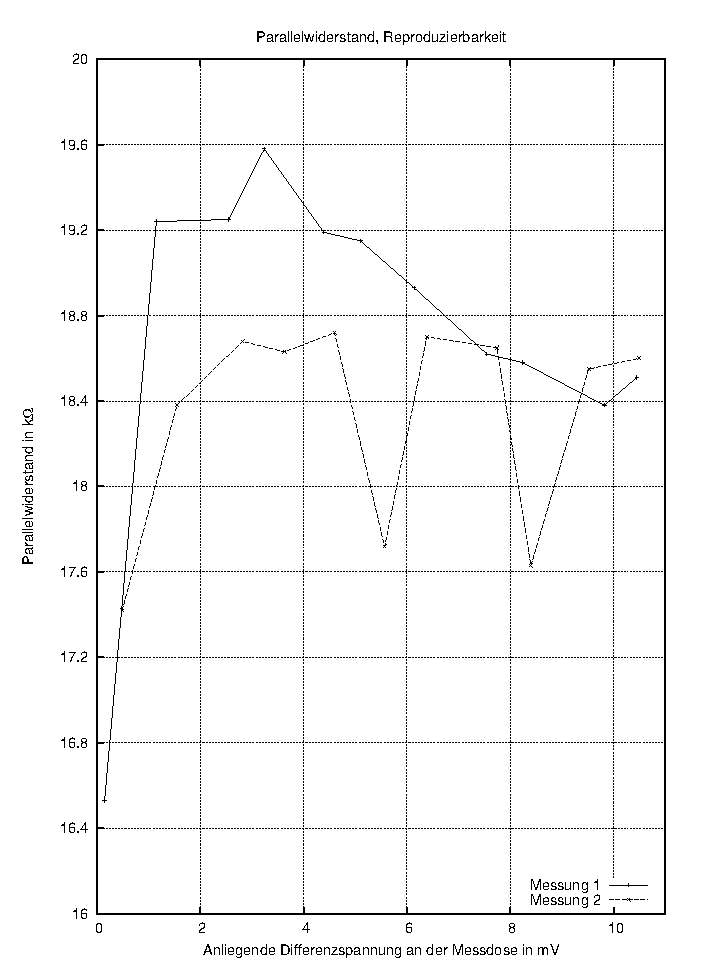
\includegraphics{tabelle2_2_3}
      \end{center}
\caption{Messung 8; mit Entladung, ohne Setz-Zeit; Piezostack; Parallelwiderstand}
\label{fig:2.8}
\end{figure}

\newpage
\subsection{Messung Piezo-Stack, mit Entladung, mit 2 Minuten Setz-Zeit}
Um eine treffen Aussage fassen zu können, wurde die vorhergehende Messung komplett wiederholt. Jedoch wurde dieses mal bei den einzelnen Werten eine Setz-Zeit von 2 Minuten eingehalten, um etwaige Fehler aufgrund des elastischen Materials der Schraubstockbacken zu minimieren. Allerdings sieht man auch hier anhand von Abbildung \vref{fig:2.9} die deutliche Abweichung zwischen den Kapazitätslinien. Die dazugehörigen Werte sind in Tabelle \vref{tab:2.9} zu finden.\\
Auch hier wurde eine Messung des auftretenden Parallelwiderstands angestoßen. Die Resultate sind in Tabelle \vref{tab:2.10} und Abbildung \vref{fig:2.10} nachzulesen.

\setlongtables
\begin{longtable}{| l | l | l | l |}
\caption{Messung 9; Piezostack; mit Entladung, 2 Minuten Setz-Zeit; Kapazität}\\
\hline
\multicolumn{2}{|c|}{Messung 1} &\multicolumn{2}{|c|}{Messung 2}\\
\hline
$U_{diff}$ in mV&$C_{Piezo}$ in nF&$U_{diff}$ in mV&$C_{Piezo}$ in nF\\
\hline
\endfirsthead
\hline
\multicolumn{2}{|c|}{Messung 1} &\multicolumn{2}{|c|}{Messung 2}\\
\hline
$U_{diff}$ in mV&$C_{Piezo}$ in nF&$U_{diff}$ in mV&$C_{Piezo}$ in nF\\
\hline
\endhead
\hline
\multicolumn{4}{|c|}{Fortsetzung auf der nächsten Seite}\\
\hline
\endfoot
\hline \hline
\endlastfoot
\hline
\label{tab:2.9}%
0.55&268.80&1.16&268.90\\
1.17&268.55&2.33&269.23\\
2.26&268.73&3.34&269.35\\
3.27&268.94&4.33&269.43\\
4.27&269.13&4.99&269.51\\
4.93&269.14&6.20&269.85\\
6.10&269.37&7.03&269.90\\
6.95&269.50&8.32&270.30\\
8.21&269.70&9.31&269.99\\
9.24&269.60&10.41&270.33\\
10.30&269.83&&\\
\end{longtable}

\begin {figure}[htbp]
      \begin{center}
        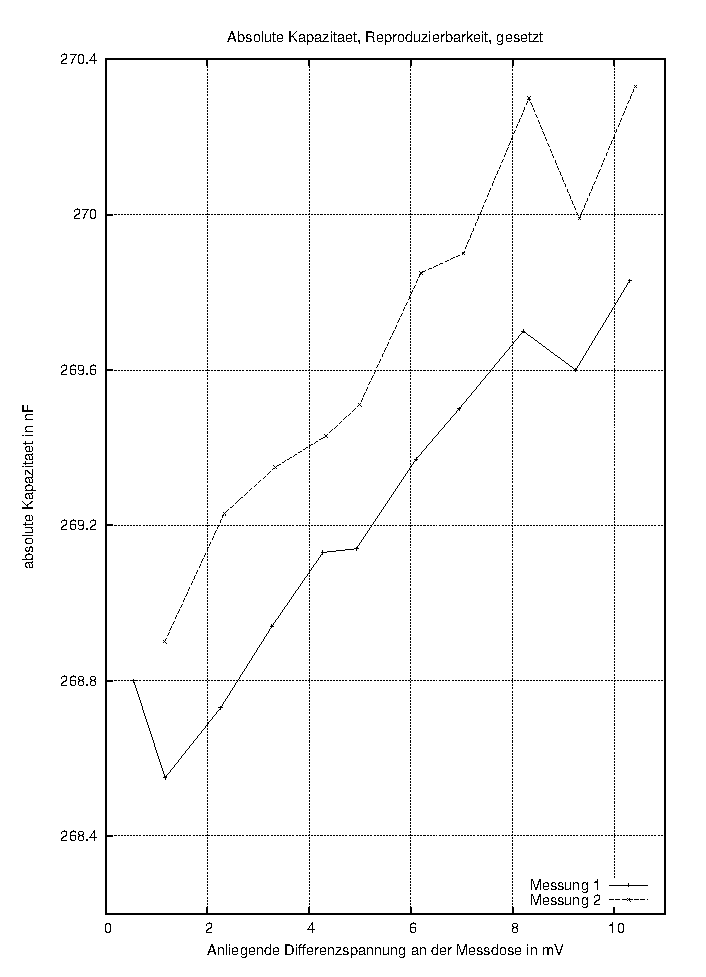
\includegraphics{tabelle2_2_4}
      \end{center}
\caption{Messung 9; mit Entladung, 2 Minuten Setz-Zeit; Piezostack; Kapazität}
\label{fig:2.9}
\end{figure}
\setlongtables
\begin{longtable}{| l | l | l | l |}
\caption{Messung 10; Piezostack; mit Entladung, 2 Minuten Setz-Zeit; Parallelwiderstand}\\
\hline
\multicolumn{2}{|c|}{Messung 1} &\multicolumn{2}{|c|}{Messung 2}\\
\hline
$U_{diff}$ in mV&$R_{Parallel}$ in k$\Omega$&$U_{diff}$ in mV&$R_{Parallel}$ in k$\Omega$\\
\hline
\endfirsthead
\hline
\multicolumn{2}{|c|}{Messung 1} &\multicolumn{2}{|c|}{Messung 2}\\
\hline
$U_{diff}$ in mV&$R_{Parallel}$ in k$\Omega$&$U_{diff}$ in mV&$R_{Parallel}$ in k$\Omega$\\
\hline
\endhead
\hline
\multicolumn{4}{|c|}{Fortsetzung auf der nächsten Seite}\\
\hline
\endfoot
\hline \hline
\endlastfoot
\hline
\label{tab:2.10}%
0.55&17.38&1.16&17.80\\
1.17&18.08&2.33&18.65\\
2.26&19.07&3.34&18.80\\
3.27&19.15&4.33&18.88\\
4.27&19.18&4.99&18.89\\
4.93&19.30&6.20&18.87\\
6.10&19.29&7.03&18.69\\
6.95&19.30&8.32&18.82\\
8.21&19.29&9.31&19.10\\
9.24&19.44&10.41&19.00\\
10.30&19.49&&\\
\end{longtable}

\begin {figure}[htbp]
      \begin{center}
        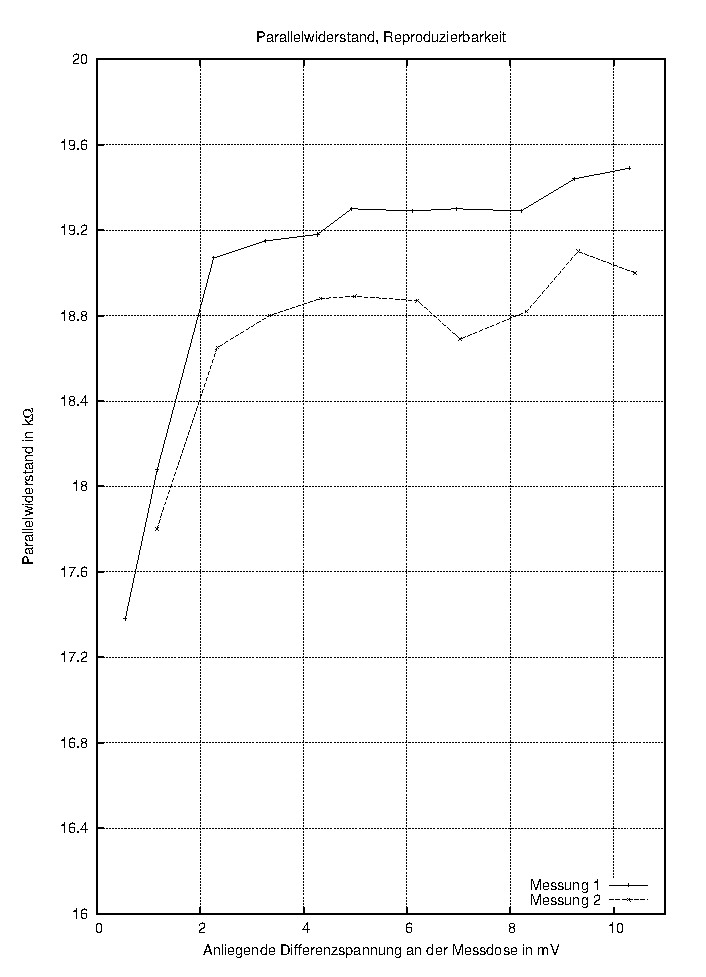
\includegraphics{tabelle2_2_5}
      \end{center}
\caption{Messung 10; mit Entladung, 2 Minuten Setz-Zeit; Piezostack; Parallelwiderstand}
\label{fig:2.10}
\end{figure}
\listoffigures
\listoftables
\end{document}
